\chapter{纯净物与混合物}\label{ch:g6:pure-substances-and-mixtures}

一瓶矿泉水的标签上列出了十二种溶解物质，
并标明了它们的含量，单位是毫克每升。
实验室净化器流出的水则什么都没有列出。
两者都清澈透明、没有颜色，都能解渴——但只有其中一种是
化学家所说的纯。本章给出“纯”这个词
确切的含义，并说明如何在不尝任何东西的前提下
区分纯净物与混合物。

\begin{recall}
混合就是把不同的东西放在一起；能溶于水的固体
溶于水后使液体保持澄清，这种澄清的液体就是溶液
（见\cref{ch:g2:mixing-and-dissolving}）。混合物可以用
筛分、倾析、过滤和蒸发
（见\cref{ch:g3:separating-mixtures}）。每种材料都有可以检验的性质：
硬或软、透明或不透明、漂浮或下沉
（见\cref{ch:g1:materials-around-us}）。
\end{recall}

\section{化学物种与纯净物}

\begin{definition}[化学物种]\label{def:g6:pure-substances-and-mixtures:species}
\emph{化学物种}\index{化学物种}是指一种特定的
物质，有其自身的名称和性质：水、糖、盐、
氧、乙醇（葡萄酒中的酒精）、铁。
\end{definition}

\begin{definition}[纯净物]\label{def:g6:pure-substances-and-mixtures:pure-substance}
\emph{纯净物}\index{纯净物}是由单一的化学物种构成的
物质，不含其他任何物质：蒸馏水、一块糖晶体、
一枚由纯金制成的金戒指。
\end{definition}

\begin{definition}[混合物]\label{def:g6:pure-substances-and-mixtures:mixture}
\emph{混合物}\index{混合物}含有多种化学物种。空气、
海水、矿泉水、牛奶、花岗岩和橙汁都是混合物。
\end{definition}

\begin{remark}[日常语言中的“纯”]\label{rem:g6:pure-substances-and-mixtures:everyday}
一盒标有“纯橙汁”的包装果汁，意思是
果汁中没有添加任何东西。在化学家看来，这种果汁仍是混合物：水、
糖类、酸、维生素、色素和香料，含有许多化学物种。“纯
山泉水”同样是混合物，它是溶有盐分的水。
\end{remark}

\begin{omfigure}
\begin{tikzpicture}[font=\small, level distance=1.55cm,
    box/.style={draw=omDef, fill=omDef!6, rounded corners=2pt, align=center,
      inner sep=4pt},
    level 1/.style={sibling distance=7.2cm},
    level 2/.style={sibling distance=3.6cm},
    edge from parent/.style={draw, thick, omDef, ->}]
  \node[box] {物质}
    child {node[box] {纯净物 \\ \footnotesize 一种化学物种}
      child {node[box, draw=black!40, fill=white] {蒸馏水、\\ 盐、铁}}}
    child {node[box] {混合物 \\ \footnotesize 含有多种化学物种}
      child {node[box] {均相 \\ \footnotesize 处处看起来一样}
        child {node[box, draw=black!40, fill=white] {盐水、\\ 空气}}}
      child {node[box] {非均相 \\ \footnotesize 可以看到不同部分}
        child {node[box, draw=black!40, fill=white] {泥水、\\ 花岗岩}}}};
\end{tikzpicture}

{\small 物质的分类。底部的方框给出了每一类的例子。}
\end{omfigure}

\section{均相混合物与非均相混合物}

\begin{definition}[均相混合物与非均相混合物]\label{def:g6:pure-substances-and-mixtures:homogeneous}
若混合物的不同部分即使借助放大镜也无法用肉眼分辨，称其为\emph{均相混合物}\index{均相混合物}，
即它处处看起来都一样。与之相对，
若混合物中至少能看到两个不同的部分，
则称其为\emph{非均相混合物}\index{非均相混合物}，
即其中的不同部分可以分辨。
\end{definition}

\begin{example}[四种混合物]\label{ex:g6:pure-substances-and-mixtures:four}
盐水和空气都是均相的：看不到它们的不同部分。水面上的油
是非均相的：分成两层。泥水是非均相的：泥粒
漂浮在水中并沉降。带果肉的橙汁是非均相的：
能看到果肉的小块。
\end{example}

\begin{omfigure}
\begin{tikzpicture}[font=\small, scale=1.15]
  \pic[transform shape] at (0,0) {beaker={0.7}{omWater!80}};
  \node[anchor=north, align=center] at (0,-0.15) {盐水：\\ 均相};
  \pic[transform shape] at (2.6,0) {beaker={0.7}{omWater!80}};
  \fill[yellow!55!orange!60] (1.8,1.05) rectangle (3.4,1.4);
  \draw[omGlass, line width=0.7pt] (1.8,1.05) -- (1.8,1.4) (3.4,1.05) -- (3.4,1.4);
  \node[anchor=north, align=center] at (2.6,-0.15) {水面上的油：\\ 非均相};
  \pic[transform shape] at (5.2,0) {beaker={0.7}{brown!25}};
  \foreach \x/\y in {4.6/0.3,4.9/0.7,5.3/0.5,5.6/1.0,5.0/1.1,5.4/0.2,5.8/0.6}
    \fill[brown!65] (\x,\y) circle (0.04);
  \fill[brown!60] (4.4,0) rectangle (6.0,0.12);
  \node[anchor=north, align=center] at (5.2,-0.15) {泥水：\\ 非均相};
  \pic[transform shape] at (7.8,0) {beaker={0.7}{orange!45}};
  \foreach \x/\y in {7.3/0.35,7.6/0.8,8.0/0.5,8.3/1.0,7.7/1.15,8.2/0.25,7.45/0.65}
    \fill[orange!80!brown] (\x,\y) ellipse (0.08 and 0.03);
  \node[anchor=north, align=center] at (7.8,-0.15) {带果肉的橙汁：\\ 非均相};
\end{tikzpicture}

{\small 一种均相混合物和三种非均相混合物。}
\end{omfigure}

\begin{omfigure}
\begin{minipage}[b]{0.48\linewidth}\centering
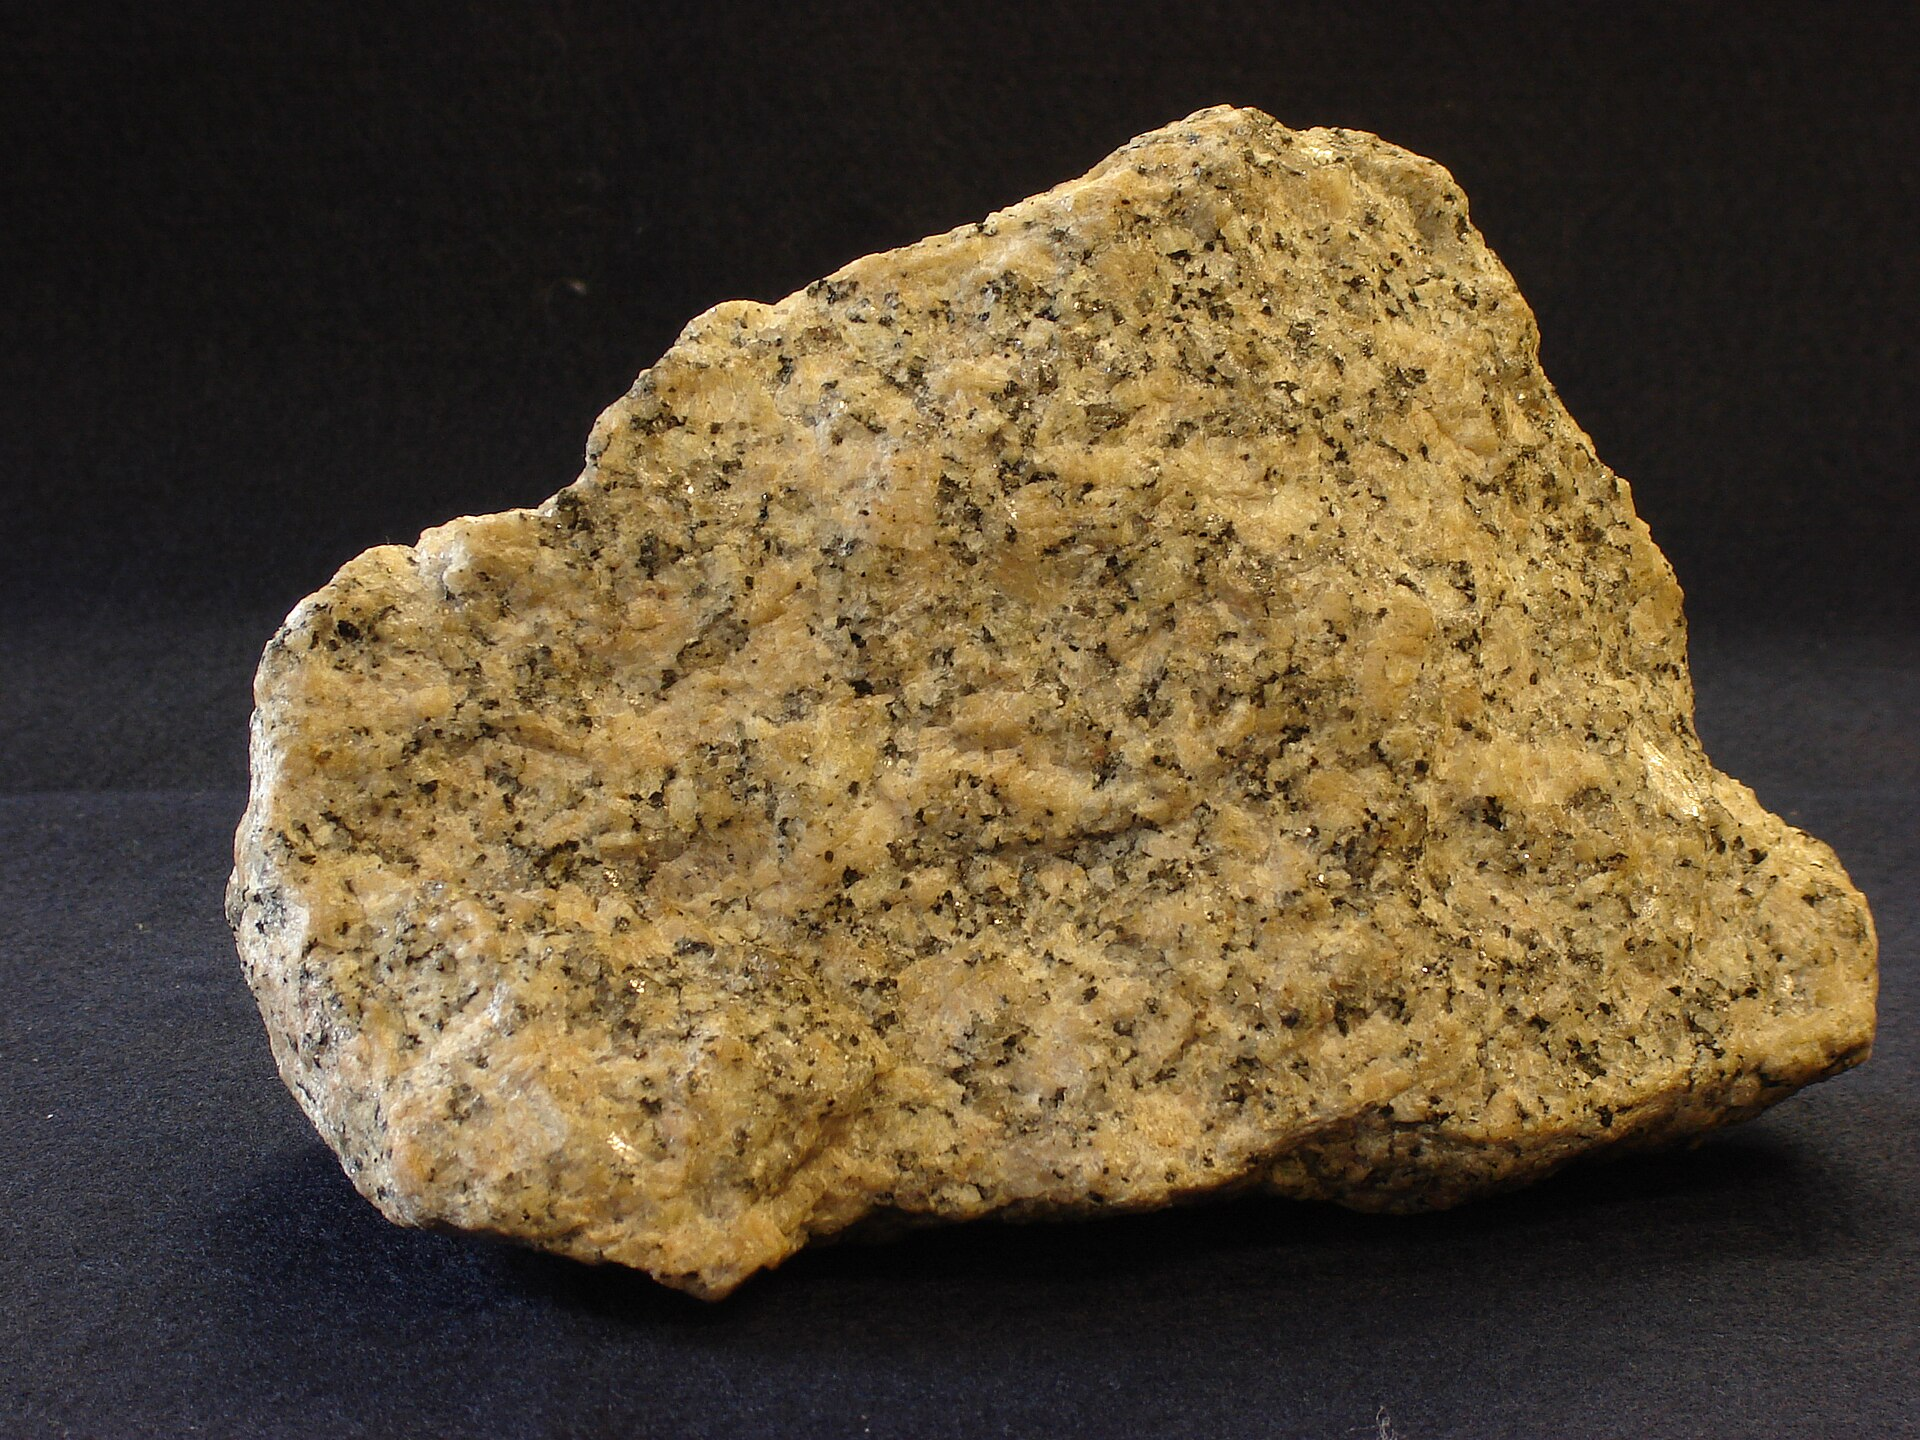
\includegraphics[width=\linewidth,height=4.6cm,keepaspectratio]{images/book1/granite.jpg}

{\small 花岗岩：可以看到三到四种不同矿物的颗粒。
这是一种非均相固体。照片：Eurico Zimbres，CC BY-SA 2.0 br.}
\end{minipage}\hfill
\begin{minipage}[b]{0.48\linewidth}\centering
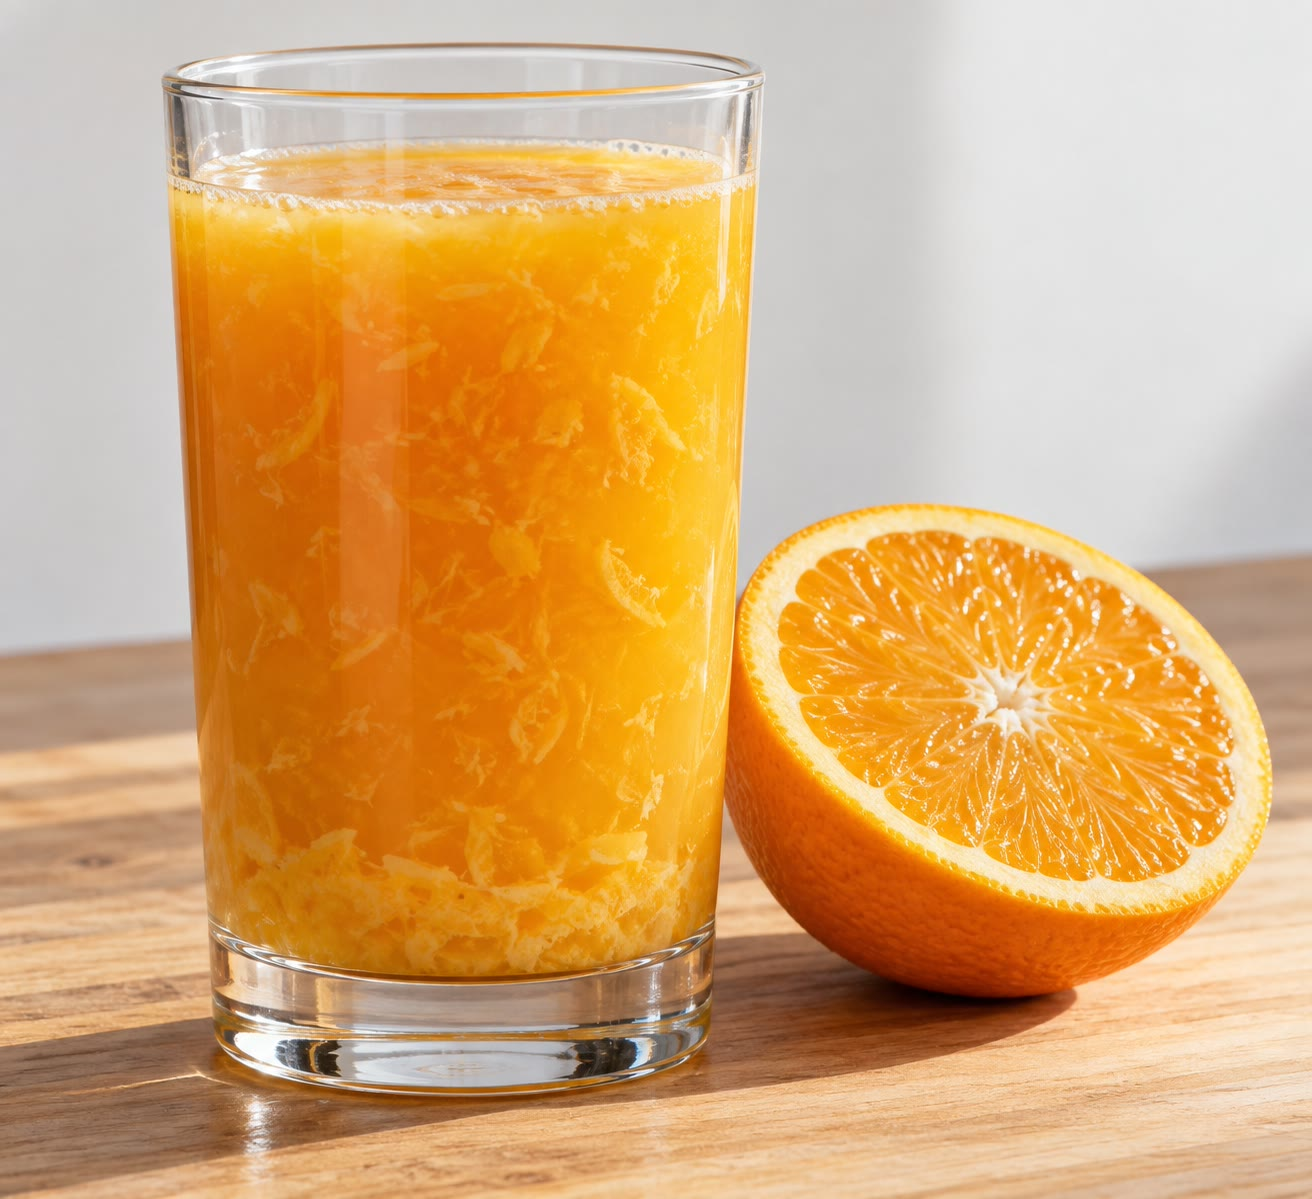
\includegraphics[width=\linewidth,height=4.6cm,keepaspectratio]{images/book1/ai/g6-orange-juice.jpg}

{\small 带果肉的橙汁：一种非均相混合物。}
\end{minipage}
\end{omfigure}

\begin{remark}[均相不等于纯净]\label{rem:g6:pure-substances-and-mixtures:not-pure}
盐水看起来与纯水一模一样。仅凭外观
不足以区分纯净物与均相混合物，必须测量某种量。
\end{remark}

\section{根据常数识别纯净物}

\begin{proposition}[纯净物有其自身的常数]\label{prop:g6:pure-substances-and-mixtures:constants}
% ledger: mp:water, bp:water, bp:ethanol, mp:ethanol, rho:water, rho:ethanol, mp:NaCl, mp:Fe, rho:Fe
每种纯净物都在各自固定的温度下熔化，
在常压下于各自固定的温度沸腾，并且
在给定体积下具有各自的质量，即密度。这些数值是它的常数；物理教材
解释了它们测量的是什么。下表列出几种纯净物的数据：
\begin{center}
\small
\begin{tabular}{lccc}
\hline
纯净物 & 熔点 & 沸点 & \qty{1}{cm^3} 的质量 \\
\hline
水 & \qty{0}{\celsius} & \qty{100}{\celsius} & 约 \qty{1.0}{g} \\
乙醇 & \qty{-114}{\celsius} & \qty{78}{\celsius} & \qty{0.79}{g} \\
丙酮 &——& \qty{56}{\celsius} & \qty{0.78}{g} \\
食盐（氯化钠） & \qty{801}{\celsius} &——& \qty{2.17}{g} \\
铁 & \qty{1538}{\celsius} &——& \qty{7.87}{g} \\
\hline
\end{tabular}
\end{center}
% ledger: bp:acetone, rho:acetone, rho:NaCl
\end{proposition}

\begin{proposition}[混合物没有固定的沸点]\label{prop:g6:pure-substances-and-mixtures:mixture-boils}
混合物没有固定的沸腾温度：盐水开始沸腾时
温度略高于 \qty{100}{\celsius}，沸腾过程中其温度持续上升，
因为水不断逸出，剩余溶液
越来越浓。
\end{proposition}

\begin{method}[这种液体是纯净物吗？是哪一种？]\label{met:g6:pure-substances-and-mixtures:identify}
\begin{enumerate}
  \item 在实验室中加热它，并在
        沸腾时读取其温度。
  \item 若温度保持不变，该液体很可能是
        纯净物：将该温度与常数表对照。
  \item 若温度持续上升，则它是混合物。
  \item 用第二个常数加以确认，例如
        已知体积的质量。
\end{enumerate}
\end{method}

\begin{inthelab}[盐水的沸腾]
老师并排加热纯水和盐水，两杯中各插
一支温度计。纯水在 \qty{100}{\celsius} 时沸腾，并且沸腾期间
温度始终保持不变。盐水在略高于
\qty{100}{\celsius} 时开始沸腾，温度计示数
每分钟都缓慢上升。
\end{inthelab}

\section{水：纯净与否}

\begin{example}[四种水]\label{ex:g6:pure-substances-and-mixtures:waters}
% ledger: sea:salinity
\begin{itemize}
  \item \textbf{蒸馏水}由实验室制得，
        几乎是纯净物，只含水，别无他物。
  \item \textbf{自来水}是均相混合物，含有少量
        溶解物质（将一滴水滴在深色盘子上晾干，
        会留下一圈白色痕迹）。
  \item \textbf{矿泉水}是均相混合物，标签上标明
        溶解物质的含量，单位为毫克每升。
  \item \textbf{海水}是均相混合物，每千克
        约含盐类 \qty{35}{g}。
\end{itemize}
\end{example}

\begin{omfigure}
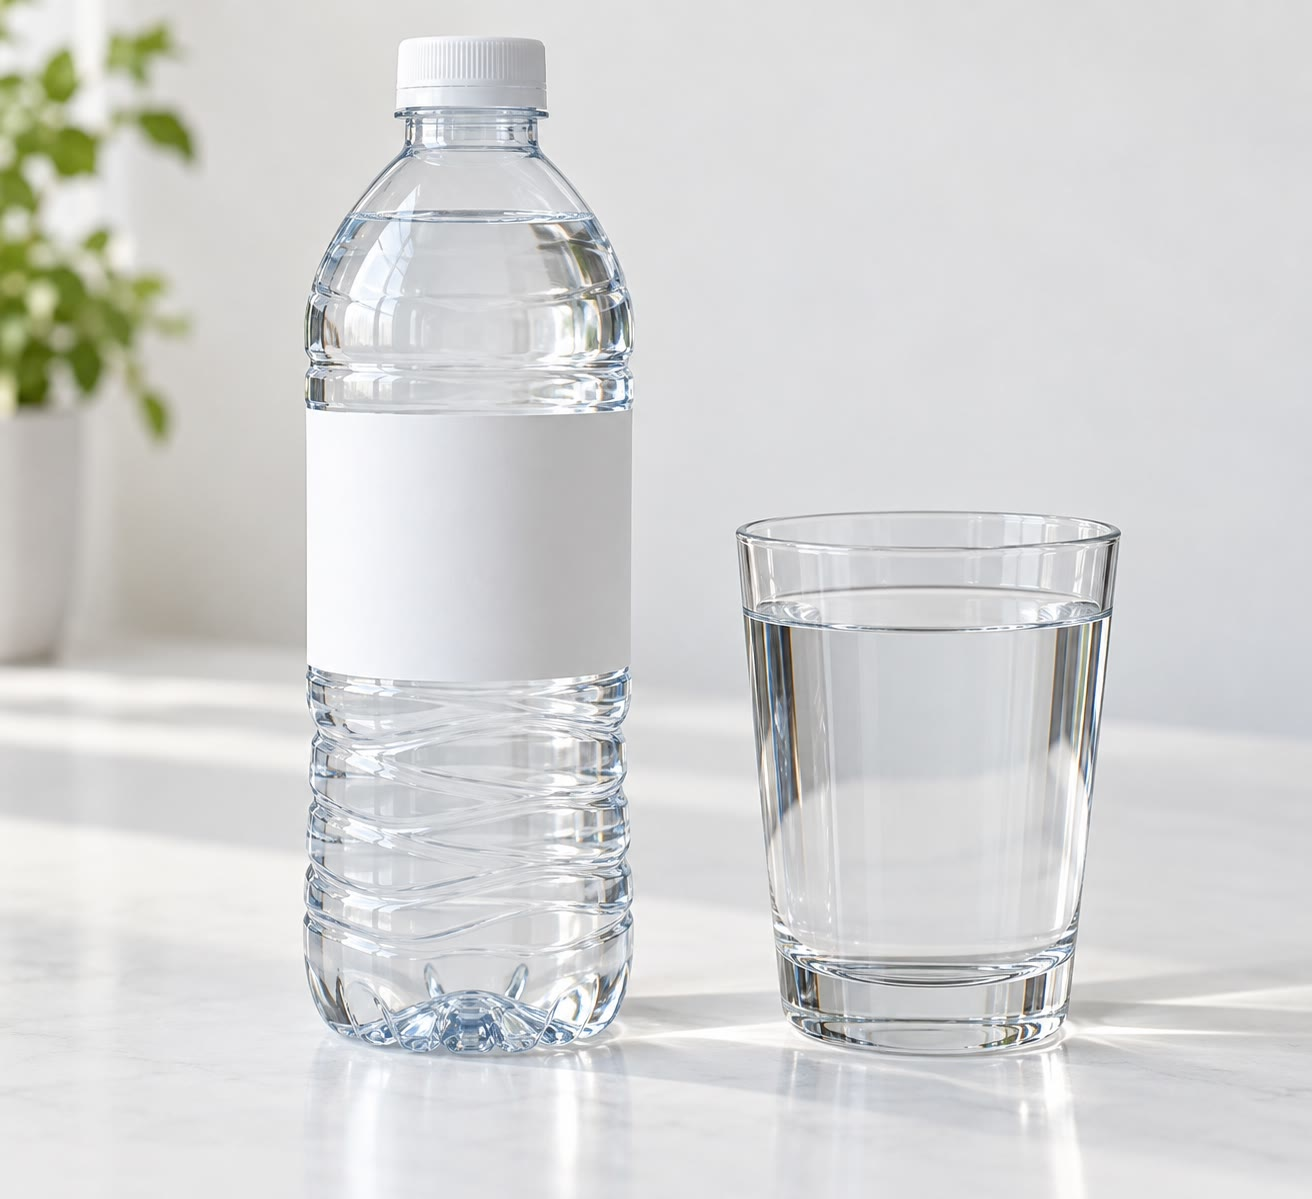
\includegraphics[width=0.5\linewidth]{images/book1/ai/g6-mineral-water.jpg}

{\small 一瓶矿泉水：清澈无色，但仍是
混合物。}
\end{omfigure}

\begin{example}[读矿泉水标签]\label{ex:g6:pure-substances-and-mixtures:label}
标签上写着：钙 \qty{78}{mg/L}、镁 \qty{24}{mg/L}、
钠 \qty{5}{mg/L}、碳酸氢根 \qty{357}{mg/L}、硫酸根
\qty{10}{mg/L}、氯离子 \qty{4}{mg/L}。（以上数据仅作示例。）
每升中溶解物质共 $78 + 24 + 5 + 357 + 10 + 4 = 478$\,mg，
约半克。与 \qty{1000}{g} 的水相比微乎其微，
但足以使它成为混合物。
\end{example}

\section{练习}

\begin{exercise}[$\star$]\label{exo:g6:pure-substances-and-mixtures:1}
判断下列物质是纯净物还是混合物：蒸馏水、空气、海水、一块
纯铁、牛奶、一粒糖晶体。
\end{exercise}

\begin{exercise}[$\star$]\label{exo:g6:pure-substances-and-mixtures:2}
判断下列物质是均相还是非均相：盐水、花岗岩、
水面上的油、自来水、什锦麦片。
\end{exercise}

\begin{exercise}[$\star$]\label{exo:g6:pure-substances-and-mixtures:3}
什么是化学物种？举出三个例子。
\end{exercise}

\begin{exercise}[$\star$]\label{exo:g6:pure-substances-and-mixtures:4}
某液体在 \qty{78}{\celsius} 时沸腾，沸腾时其温度保持在
\qty{78}{\celsius}，利用常数表推断
它可能是什么物质。
\end{exercise}

\begin{exercise}[$\star$]\label{exo:g6:pure-substances-and-mixtures:5}
为什么“纯橙汁”对化学家而言不是纯净物？
\end{exercise}

\begin{exercise}[$\star\star$]\label{exo:g6:pure-substances-and-mixtures:6}
某液体在 \qty{100.5}{\celsius} 开始沸腾，其温度
沸腾时仍会上升。它是纯净物吗？它可能是什么？
\end{exercise}

\begin{exercise}[$\star\star$]\label{exo:g6:pure-substances-and-mixtures:7}
观察四个烧杯的图。哪一个烧杯中的
混合物可用过滤法分离？哪一个不能？
\end{exercise}

\begin{exercise}[$\star\star$]\label{exo:g6:pure-substances-and-mixtures:8}
一个体积为 \qty{10}{cm^3}、质量为 \qty{78.7}{g} 的金属立方块。求
每 \qty{1}{cm^3} 的质量是多少？它可能是表中的哪种金属？
\end{exercise}

\begin{exercise}[$\star\star$]\label{exo:g6:pure-substances-and-mixtures:9}
利用例中矿泉水的标签，求碳酸氢根占溶解
物质质量的百分比，结果四舍五入到整数。
\end{exercise}

\begin{exercise}[$\star\star$]\label{exo:g6:pure-substances-and-mixtures:10}
海水每千克约含盐 \qty{35}{g}。\qty{2}{kg} 的一桶海水中
含盐多少？盐占海水质量的
百分之几？
\end{exercise}

\begin{exercise}[$\star\star\star$]\label{exo:g6:pure-substances-and-mixtures:11}
两种透明、无色的液体外观看起来完全相同。请描述在实验室中
可以进行的两种测量，用以判断它们是否为同一种
纯净物。
\end{exercise}

\begin{exercise}[$\star\star\star$]\label{exo:g6:pure-substances-and-mixtures:12}
某混合物由 \qty{90}{g} 水和 \qty{10}{g} 乙醇组成。
乙醇占其质量的百分之几？能否利用
常数表鉴别它？请说明理由。
\end{exercise}

\section{问题：三种无色液体}

\begin{problem}[{周末问题——三个无标签的透明无色液体烧瓶，
以及用于区分它们的测量}]
\label{pb:g6:pure-substances-and-mixtures:1}
% ledger: bp:water, bp:ethanol, rho:water, rho:ethanol, rho:seawater, sea:salinity
一名实验员发现三个烧瓶 A、B 和 C，其标签
均已脱落。三个烧瓶中盛的都是透明无色液体。实验室
中只使用三种此类液体：蒸馏水、乙醇，以及
从野外考察带回的海水。实验员在实验室中进行了三类
测量，均在实验室中进行。

\medskip
\noindent\textbf{第一部分——观察。}
\begin{enumerate}
  \item 三种液体外观完全相同。实验员能否仅凭
        观察判断哪些是纯净物？请说明理由。
  \item 若其中一种是混合物，它是均相还是非均相？
  \item 哪一类测量可以说明某液体
        是纯净物？
\end{enumerate}

\medskip
\noindent\textbf{第二部分——测量。}
每种液体均加热至沸腾。液体 A 在
\qty{100}{\celsius} 沸腾并保持该温度。液体 B 在
\qty{78}{\celsius} 沸腾并保持该温度。液体 C 在
\qty{100.6}{\celsius} 开始沸腾，其温度仍缓慢上升。然后
每种液体各取 \qty{50.0}{mL} 称重：A 为
\qty{49.8}{g}，B 为 \qty{39.5}{g}，C 为 \qty{51.2}{g}。
\begin{enumerate}[resume]
  \item 哪些液体是纯净物？哪一种是混合物？
  \item 利用本章常数表，说出液体 A 和
        B 的名称。
  \item 计算每种液体 \qty{1}{mL}（即 \qty{1}{cm^3}）的
        质量。
  \item 这些质量与第 5 题的答案是否一致？
  \item 液体 C 在沸腾时温度为何持续上升？
\end{enumerate}

\medskip
\noindent\textbf{第三部分——液体 C 中含有什么？}
将 \qty{100}{mL} 液体 C 置于蒸发皿中蒸干。待水分全部
蒸发后，残留 \qty{3.5}{g} 白色晶体。
\begin{enumerate}[resume]
  \item 该残留物说明液体 C 中含有什么？
  \item 利用第 6 题求得的液体 C 每 \qty{1}{mL} 的质量，求
        \qty{100}{mL} 液体 C 的质量，再求盐所占质量的
        百分比（保留一位小数）。
  \item 海水每千克约含盐 \qty{35}{g}，这相当于百分之几？
        请与第 10 题比较。
  \item 得出结论：液体 C 每升含盐多少克，
        液体 C 是否就是海水？
\end{enumerate}
\end{problem}
